% Options for packages loaded elsewhere
\PassOptionsToPackage{unicode}{hyperref}
\PassOptionsToPackage{hyphens}{url}
%
\documentclass[
  12pt,
]{article}
\usepackage{amsmath,amssymb}
\usepackage{lmodern}
\usepackage{setspace}
\usepackage{ifxetex,ifluatex}
\ifnum 0\ifxetex 1\fi\ifluatex 1\fi=0 % if pdftex
  \usepackage[T1]{fontenc}
  \usepackage[utf8]{inputenc}
  \usepackage{textcomp} % provide euro and other symbols
\else % if luatex or xetex
  \usepackage{unicode-math}
  \defaultfontfeatures{Scale=MatchLowercase}
  \defaultfontfeatures[\rmfamily]{Ligatures=TeX,Scale=1}
\fi
% Use upquote if available, for straight quotes in verbatim environments
\IfFileExists{upquote.sty}{\usepackage{upquote}}{}
\IfFileExists{microtype.sty}{% use microtype if available
  \usepackage[]{microtype}
  \UseMicrotypeSet[protrusion]{basicmath} % disable protrusion for tt fonts
}{}
\makeatletter
\@ifundefined{KOMAClassName}{% if non-KOMA class
  \IfFileExists{parskip.sty}{%
    \usepackage{parskip}
  }{% else
    \setlength{\parindent}{0pt}
    \setlength{\parskip}{6pt plus 2pt minus 1pt}}
}{% if KOMA class
  \KOMAoptions{parskip=half}}
\makeatother
\usepackage{xcolor}
\IfFileExists{xurl.sty}{\usepackage{xurl}}{} % add URL line breaks if available
\IfFileExists{bookmark.sty}{\usepackage{bookmark}}{\usepackage{hyperref}}
\hypersetup{
  pdftitle={Sensory and neural mechanisms of parent-offspring recognition in a maternal mouthbrooding African cichlid fish},
  pdfauthor={Emily Ray1*},
  hidelinks,
  pdfcreator={LaTeX via pandoc}}
\urlstyle{same} % disable monospaced font for URLs
\usepackage[margin=1in]{geometry}
\usepackage{longtable,booktabs,array}
\usepackage{calc} % for calculating minipage widths
% Correct order of tables after \paragraph or \subparagraph
\usepackage{etoolbox}
\makeatletter
\patchcmd\longtable{\par}{\if@noskipsec\mbox{}\fi\par}{}{}
\makeatother
% Allow footnotes in longtable head/foot
\IfFileExists{footnotehyper.sty}{\usepackage{footnotehyper}}{\usepackage{footnote}}
\makesavenoteenv{longtable}
\usepackage{graphicx}
\makeatletter
\def\maxwidth{\ifdim\Gin@nat@width>\linewidth\linewidth\else\Gin@nat@width\fi}
\def\maxheight{\ifdim\Gin@nat@height>\textheight\textheight\else\Gin@nat@height\fi}
\makeatother
% Scale images if necessary, so that they will not overflow the page
% margins by default, and it is still possible to overwrite the defaults
% using explicit options in \includegraphics[width, height, ...]{}
\setkeys{Gin}{width=\maxwidth,height=\maxheight,keepaspectratio}
% Set default figure placement to htbp
\makeatletter
\def\fps@figure{htbp}
\makeatother
% Make links footnotes instead of hotlinks:
\DeclareRobustCommand{\href}[2]{#2\footnote{\url{#1}}}
\setlength{\emergencystretch}{3em} % prevent overfull lines
\providecommand{\tightlist}{%
  \setlength{\itemsep}{0pt}\setlength{\parskip}{0pt}}
\setcounter{secnumdepth}{-\maxdimen} % remove section numbering
\usepackage{booktabs}
\usepackage{longtable}
\usepackage{array}
\usepackage{multirow}
\usepackage{wrapfig}
\usepackage{float}
\usepackage{colortbl}
\usepackage{pdflscape}
\usepackage{tabu}
\usepackage{threeparttable}
\usepackage{threeparttablex}
\usepackage[normalem]{ulem}
\usepackage{makecell}
\usepackage{xcolor}
\ifluatex
  \usepackage{selnolig}  % disable illegal ligatures
\fi
\newlength{\cslhangindent}
\setlength{\cslhangindent}{1.5em}
\newlength{\csllabelwidth}
\setlength{\csllabelwidth}{3em}
\newenvironment{CSLReferences}[2] % #1 hanging-ident, #2 entry spacing
 {% don't indent paragraphs
  \setlength{\parindent}{0pt}
  % turn on hanging indent if param 1 is 1
  \ifodd #1 \everypar{\setlength{\hangindent}{\cslhangindent}}\ignorespaces\fi
  % set entry spacing
  \ifnum #2 > 0
  \setlength{\parskip}{#2\baselineskip}
  \fi
 }%
 {}
\usepackage{calc}
\newcommand{\CSLBlock}[1]{#1\hfill\break}
\newcommand{\CSLLeftMargin}[1]{\parbox[t]{\csllabelwidth}{#1}}
\newcommand{\CSLRightInline}[1]{\parbox[t]{\linewidth - \csllabelwidth}{#1}\break}
\newcommand{\CSLIndent}[1]{\hspace{\cslhangindent}#1}

\title{Sensory and neural mechanisms of parent-offspring recognition in a maternal mouthbrooding African cichlid fish}
\author{Emily Ray\textsuperscript{1}*}
\date{2021-12-08 16:36:44}

\begin{document}
\maketitle

\setstretch{1.5}
\footnotesize

\textsuperscript{1}Department of Biological Sciences, Louisiana State University, Baton Rouge, LA, USA

* \textbf{Corresponding author}, email: \href{mailto:eray8@lsu.edu}{\nolinkurl{eray8@lsu.edu}}; 349 Life Science Building, Baton Rouge, LA 70803

\normalsize

\textbf{Running headline}: Cichlid offspring recognition

\textbf{Abstract}: Parental care evolved independently several times and is present in diverse taxa, from insects to mammals. Recognizing offspring is important for parental care - parents must identify and locate their young to provide resources and protection. Despite the importance of offspring recognition to species persistence, little is known about the sensory and neural mechanisms that underlie recognition in fishes, the oldest and largest group of vertebrates. Here, we identify the sensory and neural mechanisms of offspring recognition in a maternal mouthbrooding African cichlid fish, \emph{Astatotilapia burtoni}. Preliminary behavioral data suggests visual information is necessary for \emph{A. burtoni} offspring recognition, and we identify several brain regions implicated in offspring recognition. Understanding the mechanisms underlying offspring recognition in a model fish species provides insight to the evolution of parental care across vertebrate taxa, and to cichlids' response to changing environmental conditions, such as increased turbidity, that may impact their ability to send and receive sensory signals.

\clearpage

\hypertarget{introduction}{%
\section{Introduction}\label{introduction}}

Parental care has arisen from several independent evolutionary events and is present across taxa (\protect\hyperlink{ref-RN2}{Reynolds et al. 2002}, \protect\hyperlink{ref-RN1}{Gilbert and Manica 2015}). Parent-offspring recognition is critical for the maintenance of parental care because it allows parents to direct their care behaviors and energy allocation towards their own offspring, resulting in increased offspring success. Across vertebrates, parents and young rely on diverse signaling modalities for identification, including acoustic recognition in cows, chemosensory recognition in zebra finch hatchlings, and visual recognition in chimpanzees (\protect\hyperlink{ref-RN5}{Parr et al. 2010}, \protect\hyperlink{ref-RN4}{Krause et al. 2012}, \protect\hyperlink{ref-RN3}{De La Torre et al. 2016}). Recognition can also be multimodal, and can involve redundant (``same message'') or non-redundant (``different message'') signals (\protect\hyperlink{ref-RN6}{Johnstone 1996}). In some species, both parents and offspring recognize each other (bi-directional recognition), while in others, either the offspring or the parent recognizes the other (uni-directional recognition) (\protect\hyperlink{ref-RN7}{Knörnschild and Von Helversen 2008}, \protect\hyperlink{ref-RN8}{Briefer and McElligott 2011}). In fishes, both chemosensory and visual information can be important for parent-offspring recognition, and the sensory signals used vary between species (\protect\hyperlink{ref-RN9}{Neff and Sherman 2003}, \protect\hyperlink{ref-RN10}{Svensson et al. 2010}). Despite the importance of offspring recognition, how fishes, the oldest and most diverse group of vertebrates, perform this task is largely unknown.

Mouthbrooding is a form of parental care present in 53 genera of teleost fishes and 1 frog species (\protect\hyperlink{ref-RN12}{Goicoechea et al. 1986}, \protect\hyperlink{ref-RN1}{Gilbert and Manica 2015}). Mouthbrooding parents hold their developing young in their mouths and typically cease feeding behavior, starving themselves while their offspring develop (\protect\hyperlink{ref-RN11}{Oppenheimer 1970}). Despite this starvation, filial cannibalism is not common during the mouthbrooding period (\protect\hyperlink{ref-RN13}{Okuda and Yanagisawa 1996}). The maternal mouthbrooding African cichlid fish \emph{Astatotilapia burtoni} is an emerging model for neurobiology and animal behavior research that is particulary well-suited for studying parent-offspring recognition (\protect\hyperlink{ref-RN14}{Maruska and Fernald 2018}). Female \emph{A. burtoni} brood developing young in their mouths for \textasciitilde14 days, then provide post-release maternal care by collecting fry in their mouths to protect their fry from threats (\protect\hyperlink{ref-RN15}{Renn et al. 2009}). Adult \emph{A. burtoni} cannibalize fry, thus parent-offspring recognition becomes critical, both so that mothers avoid maladaptively cannibalizing their own offspring, and so that fry avoid swimming toward the wrong mouth and being consumed. However, despite the importance of parent-offspring recognition during the \emph{A. burtoni} post release maternal care phase, which sensory signals and brain regions are important for this behavior are unknown.

In the cichlid fish \emph{Pelvicachromis pulcher}, visual stimuli from fry are necessary for the maintenance of maternal care, while chemosensory stimuli from fry are not sufficient to maintain parental behaviors (\protect\hyperlink{ref-RN28}{Nelson and Elwood 1996}). However, the midas cichlid, \emph{Cichlasoma citrinellum} relies on chemosensory information for parent-offspring recognition (\protect\hyperlink{ref-RN29}{McKay and Barlow 1976}), highlighting the diverse sensory mechanisms underlying parent-offspring recognition in cichlid fishes. During the \emph{A. burtoni} post release maternal care phase, fry will attempt to enter the mouth of an adult male fish if provided only visual stimuli (\protect\hyperlink{ref-RN15}{Renn et al. 2009}), suggesting chemosensory information is necessary and non-redundant with visual information during \emph{A. burtoni} parent-offspring recognition.

The goal of this study was to determine the relative importance of visual and chemosensory signals during \emph{A. burtoni} parent-offspring recognition, and identify brain regions and networks that are important for this behavior. We compared behavior in response to different sensory stimuli from fry, and identified distinct neural activation patterns associated with parent-offspring recognition. Because fishes are the largest and oldest vertebrate group, these findings have important implications for the evolution of parental care circuits and behavior across vertebrate taxa.

\hypertarget{methods}{%
\section{Methods}\label{methods}}

\textbf{Animal Care}\\
\emph{Astatotilapia burtoni} derived from a wild-caught stock from Lake Tanganyika, Africa were laboratory raised under conditions similar to their natural environment. (\textasciitilde28 °C, pH 8.0, 12-h light/12-h dark cycle). Fish were fed cichlid flakes (AquaDine, Healdsburg, CA, USA) daily and brine shrimp (Sally's Frozen Brine Shrimp, San Francisco, CA, USA) twice weekly. Prior to experiments, fish were housed in mixed sex groups in aquaria with gravel, halved terracotta pots to serve as shelters, and several dominant males. All experimental protocols were approved by the Institutional Animal Care and Use Committee (IACUC) at Louisiana State University, Baton Rouge, LA, and were in accordance with the guidelines set by the National Institutes of Health (NIH) Guide for the Care and Use of Laboratory Animals, 2011.

\textbf{Experimental Procedures}\\
To determine the relative importance of visual and chemosensory signals in \emph{A. burtoni} offspring recognition, we compared the behavior of mouthbrooding females on the day of fry release when exposed to either 1) only visual 2)only chemosensory 3) both visual and chemosensory (C+V) or 4) no stimuli from their fry (N = 5 per condition). To obtain chemosensory stimuli, 12 fry were soaked in 250 mL of reverse osmosis filtered water for 3 hours. The fry were then removed from the water, and the water was delivered to the focal female at the start of the behavior trial via a gravity fed system with a flow rate of 3.47 mL \(s^{-1}\). Visual stimuli was the focal female's fry, visible through a clear, acrylic barrier. Behavior trials were recorded for 30 minutes and behavior was quantified using ToxTrac animal tracking software (\protect\hyperlink{ref-RN16}{Rodriguez et al. 2018}). An association index was calculated for each animal by determining the visual field of the focal animal every three minutes of the trial. If the visual field included the stimulus delivery site, the animal was scored as 1, if it did not include the stimulus delivery site, it was scored as 0. The cumulative score became the ``association score.'' This association score was then multiplied by the number of seconds in the association zone during the first 10 minutes of the trial. This product was then the ``association index.''

Immediately following behavior trials, the focal female's standard length (SL) and body mass (BM) were recorded. Each females' condition factor was calculated following the standard condition factor formula: \(CF = (W/L^3)*100\). Females were sacrificed via rapid cervical transection. Ovaries were removed and weighed to calculate gonadosomatic index (GSI). Brains were exposed and heads were fixed in 4\% paraformaldehyde at 4°C for 24 h. Heads were then transferred to 1x phosphate buffered saline (PBS) and rinsed for \textasciitilde{} 24 h at 4°C. Brains were cryoprotected in 30\% sucrose made in 1x PBS for 24 h at 4°C, embedded in optimal cutting temperature (OCT) media and sectioned in the transverse plane at 20 µm using a cryostat (Cryostar NX50), then collected on alternate sets of charged slides (VWR, Superfrost) and stored at -80°C until staining.

\textbf{pS6 Immunohistochemistry}\\
To identify activated neurons, immunohistochemistry for the phosphorylated ribosomal protein pS6 was performed, as used previously (\protect\hyperlink{ref-RN24}{Butler et al. 2018}, \protect\hyperlink{ref-RN18}{Maruska et al. 2020}). Phosphorlyation of S6 is associated with increased translation, and pS6 is present in neurons that were activated within \textasciitilde1 h prior to sacrifice (\protect\hyperlink{ref-RN27}{Ruvinsky and Meyuhas 2006}, \protect\hyperlink{ref-RN25}{Knight et al. 2012}). Slides were thawed, and sectioned tissue was surrounded with a hydrophobic barrier (Immedge Pen, Vector Laboratories). Slides were washed with 1xPBS (3 x 10 min), and non-specific binding was blocked (2\% bovine serum albumin, 0.3\% Triton-X, and 5.0\% normal goat serum, made in 1 x PBS, 2 h). Slides were incubated with pS6 antibody (1:1500; Cell Signaling Technologies pS6 ribosomal protein S235/236 antibody \#4858) overnight at 4°C. Slides were rinsed with 1xPBS (3 x 10 min), incubated with biotinylated goat anti-rabbit IgG secondary antibody (Vector Labs BA-1000; 1:277) at room temperature for 2 h, and reacted with 3,3'-diaminobenzidine (DAB, DAB Substrate Kit, Peroxidase (HRP), with Nickel Vector Laboratories SK-4100) substrate for 30 mins. Slides were rinsed in DI water (10 min) to stop the DAB reaction, then dehydrated in an ethanol series (50\%, 70\%, and 95\% EtoH 1 min, 100\% EtoH 2 x 2 min), cleared in xylene (2 x 3 min), and coverslipped with cytoseal-60 (Epredia).

\textbf{Imaging and Analysis}\\
Slide were visualized on a Nikon Eclipse Ni microscope and images were taken using a digital color camera (Nikon DS-Fi2) controlled with Nikon NIS elements software. Quantification of pS6 stained cells was performed by individuals blind to the experimental condition. Borders were drawn around regions of interest (ROI) and gridlines were applied. Boxes were randomly selected (3-5 depending on ROI size) and the number of pS6 stained cells within selected boxes was counted. pS6 stained cell density was calculated as the number of pS6 stained cells divided by the area of the boxes that were quantified. For a given region, 3-4 consecutive sections were quantified at the same location within the nucleus across animals. Data from each animal was averaged together to calculate a mean density of pS6 stained cells in each brain region.

We quantified 3 brain nuclei that are implicated in maternal care and social behavior: subdivisions 4 and 5 of the central dorsal telencephalon (Dc-4, Dc-5) and the periventricular posterior tuberculum (TPp). 100 \(\mu\)m boxes were used for the Dc-4 and Dc-5, and 50 \(\mu\)m boxes were used for the TPp.

\textbf{Statistical Analysis}\\
All analysis was performed in R 4.1.0 (\protect\hyperlink{ref-RN36}{R Core Team 2013}). Code for analysis and raw data can be accessed at \url{https://github.com/ejray21/Biol7800/tree/main/Project}.

Data was imported to R in .csv format and labeled as ``data'' using `data \textless- POR\_Master\_Sheet.' Anovas were perfomed using the format `aov(dependent variable\textasciitilde treatment).' Tukey post-hoc tests were performed to determine relationships between treatment groups using `TukeyHSD(``anova data'').'

Tables were made using the `tables' package. Figures were made using `ggplot2' `geom\_boxplot.' Individual data points were added to graphs using `geom\_jitter.'

\hypertarget{results}{%
\subsection{Results}\label{results}}

Females across all treatment groups had similar body masses, standard lengths, and condition factors (Table 1, Table 2).

Table 1. Summary of anovas comparing mass, standard length, and condition factors between treatment groups.

\begin{verbatim}
## [1] "Body Mass"
\end{verbatim}

\begin{verbatim}
##                Df Sum Sq Mean Sq F value Pr(>F)
## data$Treatment  3  0.292  0.0974    0.73   0.55
## Residuals      15  1.995  0.1330               
## 2 observations deleted due to missingness
\end{verbatim}

\begin{verbatim}
## [1] " Standard length"
\end{verbatim}

\begin{verbatim}
##                Df Sum Sq Mean Sq F value Pr(>F)
## data$Treatment  3     27     9.0    0.54   0.66
## Residuals      15    252    16.8               
## 2 observations deleted due to missingness
\end{verbatim}

\begin{verbatim}
## [1] "Condition Factor"
\end{verbatim}

\begin{verbatim}
##                Df   Sum Sq  Mean Sq F value Pr(>F)
## data$Treatment  3 5.20e-08 1.72e-08    0.21   0.89
## Residuals      15 1.22e-06 8.14e-08               
## 2 observations deleted due to missingness
\end{verbatim}

Table 2. Body Mass, Standard Length, and Condition Factor of females in each treatment group.

\begin{tabular}{lccccccc}
\hline
 &  & \multicolumn{2}{c}{Body.Mass.g} & \multicolumn{2}{c}{Standard.Length.mm} & \multicolumn{2}{c}{Condition.Factor} \\ 
treatment  & n & mean & sd & mean & sd & mean & \multicolumn{1}{c}{sd} \\ 
\hline
Control  & $\phantom{0}5$ & $\phantom{0}1.11660$ & $\phantom{0}0.52309$ & $36.40000$ & $\phantom{0}6.34823$ & $\phantom{0}0.00223$ & $\phantom{0}0.00028$ \\
Chemosensory  & $\phantom{0}5$ & $\phantom{0}1.07660$ & $\phantom{0}0.40146$ & $36.20000$ & $\phantom{0}2.94958$ & $\phantom{0}0.00219$ & $\phantom{0}0.00038$ \\
Visual  & $\phantom{0}4$ & $\phantom{0}1.36775$ & $\phantom{0}0.16102$ & $39.25000$ & $\phantom{0}1.89297$ & $\phantom{0}0.00227$ & $\phantom{0}0.00026$ \\
C + V  & $\phantom{0}5$ & $\phantom{0}1.02840$ & $\phantom{0}0.21108$ & $36.40000$ & $\phantom{0}3.36155$ & $\phantom{0}0.00212$ & $\phantom{0}0.00019$ \\
All  & $19$ & $\phantom{0}1.13574$ & $\phantom{0}0.35648$ & $36.94737$ & $\phantom{0}3.93663$ & $\phantom{0}0.00220$ & $\phantom{0}0.00027$ \\
\hline 
\end{tabular}

\textbf{Behavior}

Females exposed to only chemosensory stimuli showed a trend toward swimming farther distances than females exposed to only visual, multimodal, or no stimuli (Table 3, Figure 1). To score the female's association with the stimulus delivery site, we created an association index. Females exposed to only visual stimuli or multimodal stimuli showed a trend toward a greater association index than females exposed to only chemosensory stimuli (Table 3, Figure 2).

Table 3. Anova results for behavior data.

\begin{verbatim}
## [1] "Distance Traveled"
\end{verbatim}

\begin{verbatim}
##                Df   Sum Sq   Mean Sq F value Pr(>F)
## data$Treatment  3 6.89e+08 229699335    0.59   0.63
## Residuals      16 6.19e+09 387097073               
## 1 observation deleted due to missingness
\end{verbatim}

\begin{verbatim}
## [1] "Association index"
\end{verbatim}

\begin{verbatim}
##                Df   Sum Sq Mean Sq F value Pr(>F)
## data$Treatment  3  1542672  514224    0.72   0.56
## Residuals      16 11455470  715967               
## 1 observation deleted due to missingness
\end{verbatim}



\begin{figure}[H]

{\centering 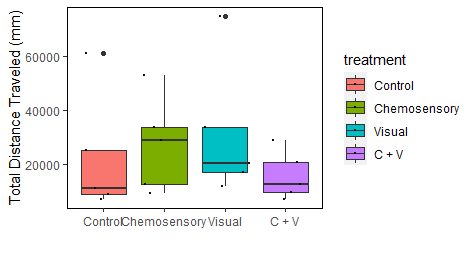
\includegraphics[width=0.7\linewidth,]{C:/Users/Owner/OneDrive - Louisiana State University/Desktop/Biol7800/Project/Figs/Figure1_Ray_FinalReport} 

}

\caption{\emph{Distance swam by females exposed to each sensory stimulus.} Females exposed to only chemosensory stimuli showed a trend toward swimming more than females that received only visual or multimodal stimuli. F3,16 = 0.59, p = 0.63, N = 5 for all groups. Boxes extend to the furthest data points of the first and third quartiles. Data median is represented by a solid line. Whiskers extend to the furthest data point within 1.5x the interquartile range. Outliers beyond 1.5x the interquartile range are represented by solid circles and are not reflective of statistical outliers.}\label{fig:fig1}
\end{figure}



\begin{figure}[H]

{\centering 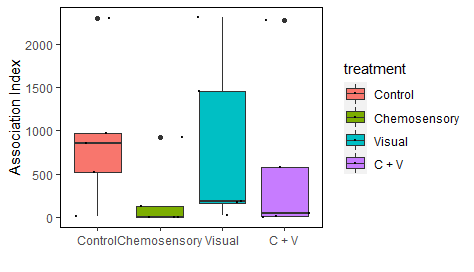
\includegraphics[width=0.7\linewidth,]{C:/Users/Owner/OneDrive - Louisiana State University/Desktop/Biol7800/Project/Figs/Fig2_AI_final report} 

}

\caption{\emph{Association index of females exposed to each set of sensory stimuli.} Females that received only chemosensory stimuli showed a trend toward a lower associaton index compared to females that received only visual stimuli or multimodal stimuli. F3,16 = 0.72, p = 0.56, N = 5 for all groups. Boxes extend to the furthest data points of the first and third quartiles. Data median is represented by a solid line. Whiskers extend to the furthest data point within 1.5x the interquartile range. Outliers beyond 1.5x the interquartile range are represented by solid circles and are not reflective of statistical outliers.}\label{fig:fig2}
\end{figure}

\textbf{Brain Activation Patterns}
Females exposed to multimodal stimuli showed a trend toward greater activation in subdivision 4 of the central dorsal telencephalon (Dc-4) compared to females exposed to unimodal or no stimuli (Table 4, Figure 3)). In subdivision 5 of the central dorsal telencephalon (Dc-5), females exposed to multimodal stimuli had greater activation than females exposed to no stimuli (Table 4, Figure 4). In the periventricular posterior tuberculum (TPp), mouthbrooders exposed to multimodal stimuli showed greater neural activation than females exposed to unimodal or no stimuli (Table 4, Figure 5).

Table 4. Anova and post-hoc results for brain activation data.

\begin{verbatim}
## [1] "Dc-4"
\end{verbatim}

\begin{verbatim}
##             Df   Sum Sq  Mean Sq F value Pr(>F)  
## treatment    3 3.17e-07 1.06e-07     3.9  0.049 *
## Residuals    9 2.44e-07 2.71e-08                 
## ---
## Signif. codes:  0 '***' 0.001 '**' 0.01 '*' 0.05 '.' 0.1 ' ' 1
\end{verbatim}

\begin{verbatim}
##   Tukey multiple comparisons of means
##     95% family-wise confidence level
## 
## Fit: aov(formula = data.dc$dc.4.cell.count ~ treatment)
## 
## $treatment
##                            diff        lwr      upr p adj
## Chemosensory-Control  0.0001907 -0.0002286 0.000610 0.519
## Visual-Control        0.0000296 -0.0003897 0.000449 0.996
## C + V-Control         0.0003762 -0.0000161 0.000768 0.061
## Visual-Chemosensory  -0.0001611 -0.0005804 0.000258 0.642
## C + V-Chemosensory    0.0001854 -0.0002068 0.000578 0.489
## C + V-Visual          0.0003465 -0.0000457 0.000739 0.086
\end{verbatim}

\begin{verbatim}
## [1] "Dc-5"
\end{verbatim}

\begin{verbatim}
##             Df   Sum Sq  Mean Sq F value Pr(>F)   
## treatment    3 2.23e-07 7.45e-08    8.62 0.0052 **
## Residuals    9 7.78e-08 8.60e-09                  
## ---
## Signif. codes:  0 '***' 0.001 '**' 0.01 '*' 0.05 '.' 0.1 ' ' 1
\end{verbatim}

\begin{verbatim}
##   Tukey multiple comparisons of means
##     95% family-wise confidence level
## 
## Fit: aov(formula = data.dc$dc.5.cell.count ~ treatment)
## 
## $treatment
##                           diff        lwr      upr p adj
## Chemosensory-Control  0.000223 -0.0000138 0.000460 0.066
## Visual-Control        0.000173 -0.0000638 0.000410 0.174
## C + V-Control         0.000358  0.0001362 0.000579 0.003
## Visual-Chemosensory  -0.000050 -0.0002869 0.000187 0.910
## C + V-Chemosensory    0.000135 -0.0000869 0.000356 0.294
## C + V-Visual          0.000185 -0.0000369 0.000406 0.109
\end{verbatim}

\begin{verbatim}
## [1] "TPp"
\end{verbatim}

\begin{verbatim}
##             Df   Sum Sq  Mean Sq F value Pr(>F)   
## treatment    3 8.19e-07 2.73e-07    9.99 0.0044 **
## Residuals    8 2.19e-07 2.73e-08                  
## ---
## Signif. codes:  0 '***' 0.001 '**' 0.01 '*' 0.05 '.' 0.1 ' ' 1
\end{verbatim}

\begin{verbatim}
##   Tukey multiple comparisons of means
##     95% family-wise confidence level
## 
## Fit: aov(formula = tpp ~ treatment)
## 
## $treatment
##                          diff       lwr      upr p adj
## Chemosensory-Control 6.67e-10 -0.000432 0.000432 1.000
## Visual-Control       6.67e-05 -0.000365 0.000499 0.958
## C + V-Control        6.22e-04  0.000190 0.001054 0.008
## Visual-Chemosensory  6.67e-05 -0.000365 0.000499 0.958
## C + V-Chemosensory   6.22e-04  0.000190 0.001054 0.008
## C + V-Visual         5.56e-04  0.000123 0.000988 0.014
\end{verbatim}



\begin{figure}[H]

{\centering 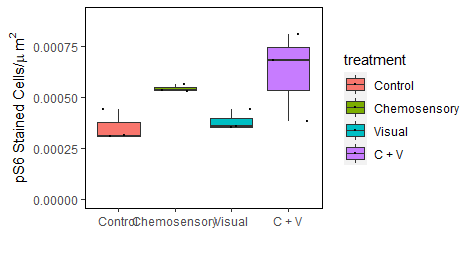
\includegraphics[width=0.7\linewidth,]{C:/Users/Owner/OneDrive - Louisiana State University/Desktop/Biol7800/Project/Figs/fig3_dc4_final Project} 

}

\caption{\emph{Neural activation in subdivision 4 of the central dorsal telencephalon (Dc-4)}. Females exposed to multimodal stimuli showed a trend toward greater activation compared to females exposed to no stimuli or multimodal stimuli. F3,9 = 3.905, p = 0.0487, N = 3 for all groups. Boxes extend to the furthest data points of the first and third quartiles. Data median is represented by a solid line. Whiskers extend to the furthest data point within 1.5x the interquartile range. Outliers beyond 1.5x the interquartile range are represented by solid circles and are not reflective of statistical outliers.}\label{fig:fig3}
\end{figure}



\begin{figure}[H]

{\centering \includegraphics[width=0.7\linewidth,]{C:/Users/Owner/OneDrive - Louisiana State University/Desktop/Biol7800/Project/Figs/fig4_dc5_Final Report} 

}

\caption{\emph{Neural activation in subdivision 5 of the central dorsal telencephalon (Dc-5)}. Females exposed to multimodal stimuli had greater activation compared to females exposed to no stimuli. F3,9 = 8.62, p = 0.00519, N = 3 for all groups. Boxes extend to the furthest data points of the first and third quartiles. Data median is represented by a solid line. Whiskers extend to the furthest data point within 1.5x the interquartile range. Outliers beyond 1.5x the interquartile range are represented by solid circles and are not reflective of statistical outliers.}\label{fig:fig4}
\end{figure}



\begin{figure}[H]

{\centering 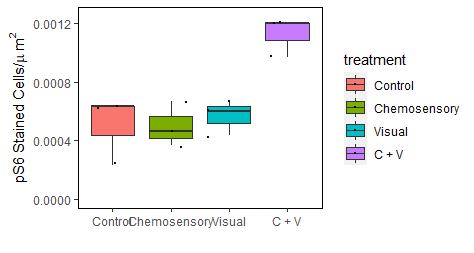
\includegraphics[width=0.7\linewidth,]{C:/Users/Owner/OneDrive - Louisiana State University/Desktop/Biol7800/Project/Figs/fig5_tpp_ray final report} 

}

\caption{\emph{Neural activation in the periventricular posterior tuberculum (TPp)}. Females exposed to multimodal stimuli had greater activation compared to females exposed to unimodal or no stimuli. F3,8 = 9.993, p = 0.00442, N = 3 for all groups. Boxes extend to the furthest data points of the first and third quartiles. Data median is represented by a solid line. Whiskers extend to the furthest data point within 1.5x the interquartile range. Outliers beyond 1.5x the interquartile range are represented by solid circles and are not reflective of statistical outliers.}\label{fig:fig5}
\end{figure}

\hypertarget{discussion}{%
\subsection{Discussion}\label{discussion}}

In behavior trials, females exposed to only chemosensory stimuli from their fry showed a trend toward swimming farther than females exposed to no stimuli, only visual stimuli, or multimodal stimuli. In contrast, females exposed to either only visual or multimodal stimuli showed a trend toward a higher association index than females exposed to only chemosensory stimuli. These trends could suggest that while chemosensory stimuli is enough to initiate searching behaviors, shown by an increase in distance swam, chemosensory stimuli alone is not sufficient for correct fry location, shown by a greater association index. The West African cichlid \emph{Pelvicachromis pulcher} similarly requires visual information for the maitenance of parental care (\protect\hyperlink{ref-RN28}{Nelson and Elwood 1996}) while fry of the more evolutionarily distant South African cichlid \emph{Amphilophus citrinellus} can recognize parents from chemosensory signals alone (\protect\hyperlink{ref-RN29}{McKay and Barlow 1976}). However, both these cichlid species are substrate brooders and thus parent-offspring recognition evolved in these species under different conditions than in mouthbrooding \emph{A. burtoni}.

Different sensory signals from fry resulted in different brain activation patterns in mouthbrooding \emph{A. burtoni}. While brain regions associated with kin recognition have been identified in zebrafish (\protect\hyperlink{ref-RN30}{Gerlach and Wullimann 2021}), to our knowledge this is the first study to identify the neural correlates of parent-offspring recognition in a fish. Females exposed to multimodal stimuli had greater neural activation, shown by greater pS6 stained cell density, compared to females that received no stimuli in Dc-5 and in Dc-4 showed a trend toward greater activation compared to females that received no stimuli or unimodal stimuli. Previous work has identified Dc-5 as being implicated in maternal care in \emph{A. burtoni} (\protect\hyperlink{ref-RN18}{Maruska et al. 2020}), suggesting it may be important for recognition of offspring and maitanence of maternal behaviors. While there is not yet consensus on the mammalian homologue for the central dorsal telencephalon, some evidence suggests it may be homologous to the mammalian neocortex (\protect\hyperlink{ref-RN31}{Mueller et al. 2011}, \protect\hyperlink{ref-RN32}{Northcutt 2011}). The mammalian neocortex is involved in functions such as motor control, sensory processing, and spatial reasoning, all of which are important functions for identification and location of offspring.

In the TPp, females that received multimodal stimuli had greater activation than females that received no stimuli or unimodal stimuli. The TPp has previously been implicated in \emph{A. burtoni} maternal care (\protect\hyperlink{ref-RN18}{Maruska et al. 2020}) and is thought to be part of the teleost social decision making network (SDMN) (\protect\hyperlink{ref-RN33}{O'Connell and Hofmann 2012}). The SDMN is made up of the social behavior network and the mesolimbic reward system and contains conserved nuclei that are though to faciliate social behaviors across vertebrates (\protect\hyperlink{ref-RN33}{O'Connell and Hofmann 2012}). The TPp is likely homologous to the mammalian ventral tegmental area (VTA) (\protect\hyperlink{ref-RN34}{Luo et al. 2008}). Dopaminergic cells in the VTA have been implicated in rodent pup retrieval during maternal care (\protect\hyperlink{ref-RN22}{Numan and Stolzenberg 2009}, \protect\hyperlink{ref-RN20}{Fang et al. 2018}) and dopamine cells are present in the TPp (\protect\hyperlink{ref-RN35}{O'Connell et al. 2011}), though whether dopamine in the TPp is conserved to faciliate fry retrieval in teleost fish is unkown.

Because these data are still preliminary, different or clearer trends may emerge as more data is collected. As we continue this experiment, we will continue to collect behavioral and neural activation data from mothers, and collect behavioral and neural activation data from fry that are exposed to the same suite of stimuli from their mothers. As neural activation data from more nuclei are collected, we will perform multivariate analyses (e.g.~PCA, differential function analysis) to identify networks of nuclei that are important for \emph{A. burtoni} parent offspring recognition.

\hypertarget{conclusions}{%
\subsection{Conclusions}\label{conclusions}}

Here, we identify three brain regions implicated in offspring recognition in a model mouthbrooding cichlid fish. To our knowledge, this is the first study to identify the neural mechanisms underlying parent-offspring recognition in a mouthbrooding fish. Because fishes are the oldest and largest group of vertebrates, identifying these mechanisms is important for our understanding of the evolution of parental care across vertebrates. Further, understanding the functions of teleost brain regions can aid in identifying brain homologies between fishes and other vertebrates. Because parental care is critical for species persistence, understanding how it is regulated in a model cichlid species is important for conservation efforts as we can better predict how parental care will be impacted by changing environmental conditions, such as pollution, warming, turbidity, and extreme weather, that may impact cichlids' ability to send and receive sensory signals.

\hypertarget{references}{%
\section*{References}\label{references}}
\addcontentsline{toc}{section}{References}

\hypertarget{refs}{}
\begin{CSLReferences}{1}{0}
\leavevmode\hypertarget{ref-RN8}{}%
Briefer, E., and A. G. McElligott. 2011. Mutual mother--offspring vocal recognition in an ungulate hider species (capra hircus). Animal cognition 14:585--598.

\leavevmode\hypertarget{ref-RN24}{}%
Butler, J. M., S. M. Whitlow, D. A. Roberts, and K. P. Maruska. 2018. Neural and behavioural correlates of repeated social defeat. Scientific reports 8:1--13.

\leavevmode\hypertarget{ref-RN3}{}%
De La Torre, M. P., E. F. Briefer, B. M. Ochocki, A. G. McElligott, and T. Reader. 2016. Mother--offspring recognition via contact calls in cattle, bos taurus. Animal Behaviour 114:147--154.

\leavevmode\hypertarget{ref-RN20}{}%
Fang, Y.-Y., T. Yamaguchi, S. C. Song, N. X. Tritsch, and D. Lin. 2018. A hypothalamic midbrain pathway essential for driving maternal behaviors. Neuron 98:192--207. e10.

\leavevmode\hypertarget{ref-RN30}{}%
Gerlach, G., and M. F. Wullimann. 2021. Neural pathways of olfactory kin imprinting and kin recognition in zebrafish. Cell and tissue research:1--15.

\leavevmode\hypertarget{ref-RN1}{}%
Gilbert, J. D., and A. Manica. 2015. The evolution of parental care in insects: A test of current hypotheses. Evolution 69:1255--1270.

\leavevmode\hypertarget{ref-RN12}{}%
Goicoechea, O., O. Garrido, and B. Jorquera. 1986. Evidence for a trophic paternal-larval relationship in the frog rhinoderma darwinii. Journal of Herpetology:168--178.

\leavevmode\hypertarget{ref-RN6}{}%
Johnstone, R. A. 1996. Multiple displays in animal communication:{`backup signals'} and {`multiple messages.'} Philosophical Transactions of the Royal Society of London. Series B: Biological Sciences 351:329--338.

\leavevmode\hypertarget{ref-RN25}{}%
Knight, Z. A., K. Tan, K. Birsoy, S. Schmidt, J. L. Garrison, R. W. Wysocki, A. Emiliano, M. I. Ekstrand, and J. M. Friedman. 2012. Molecular profiling of activated neurons by phosphorylated ribosome capture. Cell 151:1126--1137.

\leavevmode\hypertarget{ref-RN7}{}%
Knörnschild, M., and O. Von Helversen. 2008. Nonmutual vocal mother--pup recognition in the greater sac-winged bat. Animal Behaviour 76:1001--1009.

\leavevmode\hypertarget{ref-RN4}{}%
Krause, E. T., O. Krüger, P. Kohlmeier, and B. A. Caspers. 2012. Olfactory kin recognition in a songbird. Biology letters 8:327--329.

\leavevmode\hypertarget{ref-RN34}{}%
Luo, G. R., Y. Chen, X. P. Li, T. X. Liu, and W. D. Le. 2008. Nr4a2 is essential for the differentiation of dopaminergic neurons during zebrafish embryogenesis. Molecular and Cellular Neuroscience 39:202--210.

\leavevmode\hypertarget{ref-RN18}{}%
Maruska, K. P., J. M. Butler, K. E. Field, C. Forester, and A. Augustus. 2020. Neural activation patterns associated with maternal mouthbrooding and energetic state in an african cichlid fish. Neuroscience 446:199--212.

\leavevmode\hypertarget{ref-RN14}{}%
Maruska, K. P., and R. D. Fernald. 2018. Astatotilapia burtoni: A model system for analyzing the neurobiology of behavior. ACS chemical neuroscience 9:1951--1962.

\leavevmode\hypertarget{ref-RN29}{}%
McKay, KR, and G. Barlow. 1976. Chemical recognition of young by the midas cichlid, cichlasoma citrinellum. Copeia 2:276--282.

\leavevmode\hypertarget{ref-RN31}{}%
Mueller, T., Z. Dong, M. A. Berberoglu, and S. Guo. 2011. The dorsal pallium in zebrafish, danio rerio (cyprinidae, teleostei). Brain research 1381:95--105.

\leavevmode\hypertarget{ref-RN9}{}%
Neff, B. D., and P. W. Sherman. 2003. Nestling recognition via direct cues by parental male bluegill sunfish (lepomis macrochirus). Animal cognition 6:87--92.

\leavevmode\hypertarget{ref-RN28}{}%
Nelson, C., and R. Elwood. 1996. Parental state and offspring recognition in the biparental cichlid fish pevicachromis pulcher. Animal Behavior 54:803--809.

\leavevmode\hypertarget{ref-RN32}{}%
Northcutt, R. G. 2011. Do teleost fishes possess a homolog of mammalian isocortex? Brain, behavior and evolution 78:136.

\leavevmode\hypertarget{ref-RN22}{}%
Numan, M., and D. S. Stolzenberg. 2009. Medial preoptic area interactions with dopamine neural systems in the control of the onset and maintenance of maternal behavior in rats. Frontiers in neuroendocrinology 30:46--64.

\leavevmode\hypertarget{ref-RN35}{}%
O'Connell, L. A., M. R. Fontenot, and H. A. Hofmann. 2011. Characterization of the dopaminergic system in the brain of an african cichlid fish, astatotilapia burtoni. Journal of Comparative Neurology 519:75--92.

\leavevmode\hypertarget{ref-RN33}{}%
O'Connell, L. A., and H. A. Hofmann. 2012. Evolution of a vertebrate social decision-making network. Science 336:1154--1157.

\leavevmode\hypertarget{ref-RN13}{}%
Okuda, N., and Y. Yanagisawa. 1996. Filial cannibalism by mouthbrooding males of the cardinal fish, apogon doederleini, in relation to their physical condition. Environmental Biology of Fishes 45:397--404.

\leavevmode\hypertarget{ref-RN11}{}%
Oppenheimer, J. R. 1970. Mouthbreeding in fishes. Animal Behaviour 18:493--503.

\leavevmode\hypertarget{ref-RN5}{}%
Parr, L. A., M. Heintz, E. Lonsdorf, and E. Wroblewski. 2010. Visual kin recognition in nonhuman primates:(pan troglodytes and macaca mulatta): Inbreeding avoidance or male distinctiveness? Journal of Comparative Psychology 124:343.

\leavevmode\hypertarget{ref-RN36}{}%
R Core Team. 2013. R: A language and environment for statistical computing. R Foundation for Statistical Computing, Vienna, Austria.

\leavevmode\hypertarget{ref-RN15}{}%
Renn, S. C., J. B. Carleton, H. Magee, M. L. T. Nguyen, and A. C. Tanner. 2009. Maternal care and altered social phenotype in a recently collected stock of astatotilapia burtoni cichlid fish. Integrative and comparative biology 49:660--673.

\leavevmode\hypertarget{ref-RN2}{}%
Reynolds, J. D., N. B. Goodwin, and R. P. Freckleton. 2002. Evolutionary transitions in parental care and live bearing in vertebrates. Philosophical Transactions of the Royal Society of London. Series B: Biological Sciences 357:269--281.

\leavevmode\hypertarget{ref-RN16}{}%
Rodriguez, A., H. Zhang, J. Klaminder, T. Brodin, P. L. Andersson, and M. Andersson. 2018. ToxTrac: A fast and robust software for tracking organisms. Methods in Ecology and Evolution 9:460--464.

\leavevmode\hypertarget{ref-RN27}{}%
Ruvinsky, I., and O. Meyuhas. 2006. Ribosomal protein S6 phosphorylation: From protein synthesis to cell size. Trends in biochemical sciences 31:342--348.

\leavevmode\hypertarget{ref-RN10}{}%
Svensson, O., M. Lissåker, and K. B. Mobley. 2010. Offspring recognition and the influence of clutch size on nest fostering among male sand gobies, pomatoschistus minutus. Behavioral ecology and sociobiology 64:1325--1331.

\end{CSLReferences}

\end{document}
